\chapter{Neutrinoforschung} 
    \vspace{8pt}
    \section{Das Neutrino}
    Das Neutrino ist ein subatomares Teilchen der Leptonenklasse. Das Neutrino hat keine 
    elektrische Ladung und unterliegt somit nur der schwachen Wechselwirkung und der Massenanziehungkraft. 
    Nach dem Standardmodell ist das Neutrino ein punktförmiges Teilchen. Es gibt 3 Generationen 
    von Neutrinos mit jeweils anderer Masse. Da Neutrinos ein Spin von $\frac{1}{2}$ haben, sind sie Fermionen. \\ \cite{Stoecker2000} 
    \begin{center}
        \begin{tabular}{ | l | c | } \hline
            Bezeichnung & Masse (MeV) \\ \hline
            Elektron-Neutrino & >7,3 $\cdot 10^{-6}$\\ 
            Muon-Neutrino & <0,27  \\ 
            Tau-Neutrino & <31 \\ \hline
        \end{tabular}             
    \end{center} 
    Es gilt zu beachten, dass die Masse noch nicht genau bestimmt wurde, 
    doch es konnten bisher Obergrenzen bestimmt werden.\\
    Kosmische, solare, atmosphärische oder Geoneutrinos entstammen aus natürlichen Quellen / Reaktionen.
    Aus künstlichen Quellen / Reaktionen entstammen Reaktorneutrinos und Beschleunigerneutrinos. \\
    Neutrinos könnten Anwendung finden in der Reaktorkontrolle bei der Überprüfung der Plutoniumproduktion, indem 
    man die Antineutrinoemissionen misst. \cite{Krauter2006} 
    Insbesonders in der Astrophysik sind die Neutrinos von hoher Bedeutung. 
    Da sie nur schwach wechselwirken durchdringen sie fast jede Materie und so kann durch Neutrinos Bereiche 
    untersuchen die man mit anderer Strahlung nicht untersuchen kann.
    Zudem ist die Masse von Neutrinos bedeutend für viele astrophysikalische Theorien. \cite{Gelmini2010}
    Die Forschungsstätte IceCube hat eine besondere Rolle in der Untersuchung von kosmischen Neutrinos.
    \section{Geschichte} 
    \subsection{$\beta^{-}$ Zerfall} 
    Beim $\beta^{-}$-Zerfall gibt es folgende Reaktion:
    \begin{center}
    $n \rightarrow p + e^- + \overline{\nu}_e$
    \end{center}
    Doch bevor das Neutrino entdeckt wurde, sah der beobachtete $\beta^{-}$-Zerfall so aus:
    \begin{center}
    $n \rightarrow p + e^-$
    \end{center} 
    Beim Beispiel des Tritium-Zerfall ist der Verfall wie folgt:
    \begin{center}
    $\isotope[3][1]{H} \rightarrow \isotope[3][2]{He} + + e^-$
    \end{center}
    Nach dem Energiehaltungssatz, gilt:
    \begin{center}
    $ E_H = E_{He} + E_e $
    \end{center}
    Die Energie eines Teilchen kann man mit der Formel $E=c\cdot\sqrt{m^2c^2+p^2}$ bestimmen. Wir gehen 
    davon aus, dass das Neutron kein Impuls hat aufgrund der Laborbedingungen. $p_n = 0$
    Aufgrund der Impulserhaltung ergibt sich folgendes:
    \begin{flalign*}
        p_H &= p_{He} + p_e \\
        0 &= p_{He} + p_e \hspace{15pt}| -p_e\\
        - p_e &= p_{He}
    \end{flalign*}
    Die Energie vor dem Zerfall muss, der nach dem Zerfall gleichen, also
    \begin{flalign*}
        E_H &= E_p + E_e \\
        m_H\cdot c^2 &= c\cdot\sqrt{m_{He}^2c^2+p_{He}^2} + E_e \hspace{15pt}| -E_e \hspace{15pt}| ^2  \\
        (m_nc^2 -E_e )^2 &= c^2 (m_{He}^2c^2+p_{He}^2) \hspace{15pt}| -p_{He}^2  \\
        m_H^2\cdot c^2 - 2m_HE_e + \frac{E_e^2}{c^2} - p_{He}^2 &= m_{He}^2c^2 \\
        m_H^2\cdot c^2 - 2m_HE_e + \frac{E_e^2}{c^2} - p_e^2 &= m_{He}^2c^2 \\
    \end{flalign*}

    Man kann $\frac{E_e^2}{c^2} -p_e^2$ ersetzen mit einer ungeformten Formel für die Gesamtenergie
    \begin{flalign*}
        E_e &= c\cdot\sqrt{m_e^2c^2+p_e^2} \hspace{15pt}|^2 \hspace{15pt} |:c^2 \hspace{15pt} |-p_e^2 \\
        \frac{E_e^2}{c^2} -p_e^2 &= m_e^2c^2
    \end{flalign*}

    Nach $E_e$aufgelöst ist die Formel wie folgt:
    \begin{flalign*}
        m_H^2c^2 - 2m_HE_e + m_e^2c^2 &= m_{He}^2c^2 \hspace{15pt}| - m_{He}^2c^2 \hspace{15pt}| +2m_HE_e \hspace{15pt}| :2m_H \\
        c^2 \frac{m_H^2+m_e^2-m_{He}^2}{2m_H} &= E_e \\ 
        E_e &= c^2 \frac{3,0160492^2u-3,0160293^2u+0.51^2 \frac{MeV}{c^2}}{2 \cdot 3,0160293u} \\
        E_e &= 18,5 keV
    \end{flalign*} 
    Es müsste sich somit beim Energiespektrum des Tritiumzerfall eine konstante Energie von 18,5 keV ergeben.
    Dies war jedoch nicht der Fall.\cite{Horak2015}
    \begin{center}
        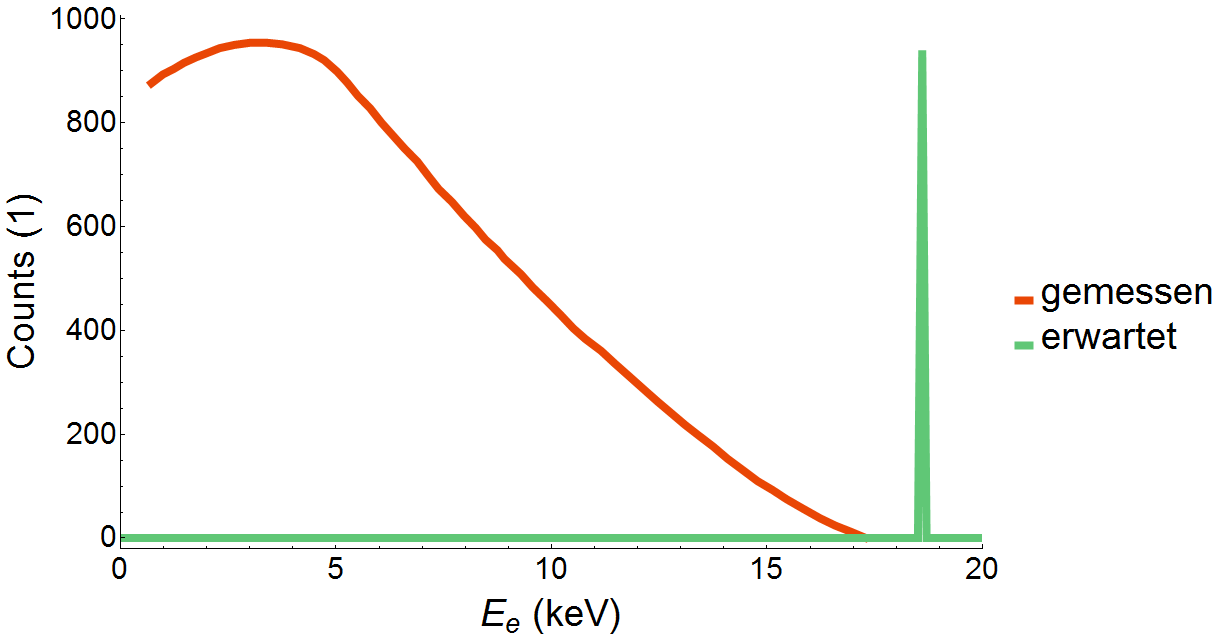
\includegraphics[width=1\textwidth]{images/Tritiumzerfall-elektronenergiespektrum}
    \end{center}
    Wie man sieht, geht Energie verloren. Anhand dieses Spektrum wusste man die maximal verlorene 
    Energie der berechneten gleich ist.
    Die erste mit dem Energiehaltungssatz konforme Erklärung für dieses Phänomen kam mit einem Brief von 
    Pauli, welcher an die "radioaktiven Damen und Herren", so bezeichnete er die Teilnehmer der 
    Gauverein-Tagung zu Tübingen, gerichtet war.
    Im Brief legt er die Vermutung nahe, dass dieser Energiespektrum aufgrund eines weiteren Teilchen entsteht. \cite{Pauli1930}
    Für Jahre konnte man keine Messung durchführen, welche dieses Teilchen beweisen würde. Das postulierte Teilchen
    sollte aber elektrisch neutral sein und nur schwach wechselwirken.
    \subsection{Reines-Cowan-Experiment}
    \section{Aktuelle Forschung}
    \section{Zukünftige Forschung}
    \section{Forschung am IceCube}